\subsection*{\textit{\textbf{RQ1: How often are addressed issues prevented from being
released?}}}\label{resutls:rq1}

\begin{figure}[!t]
	\centering
	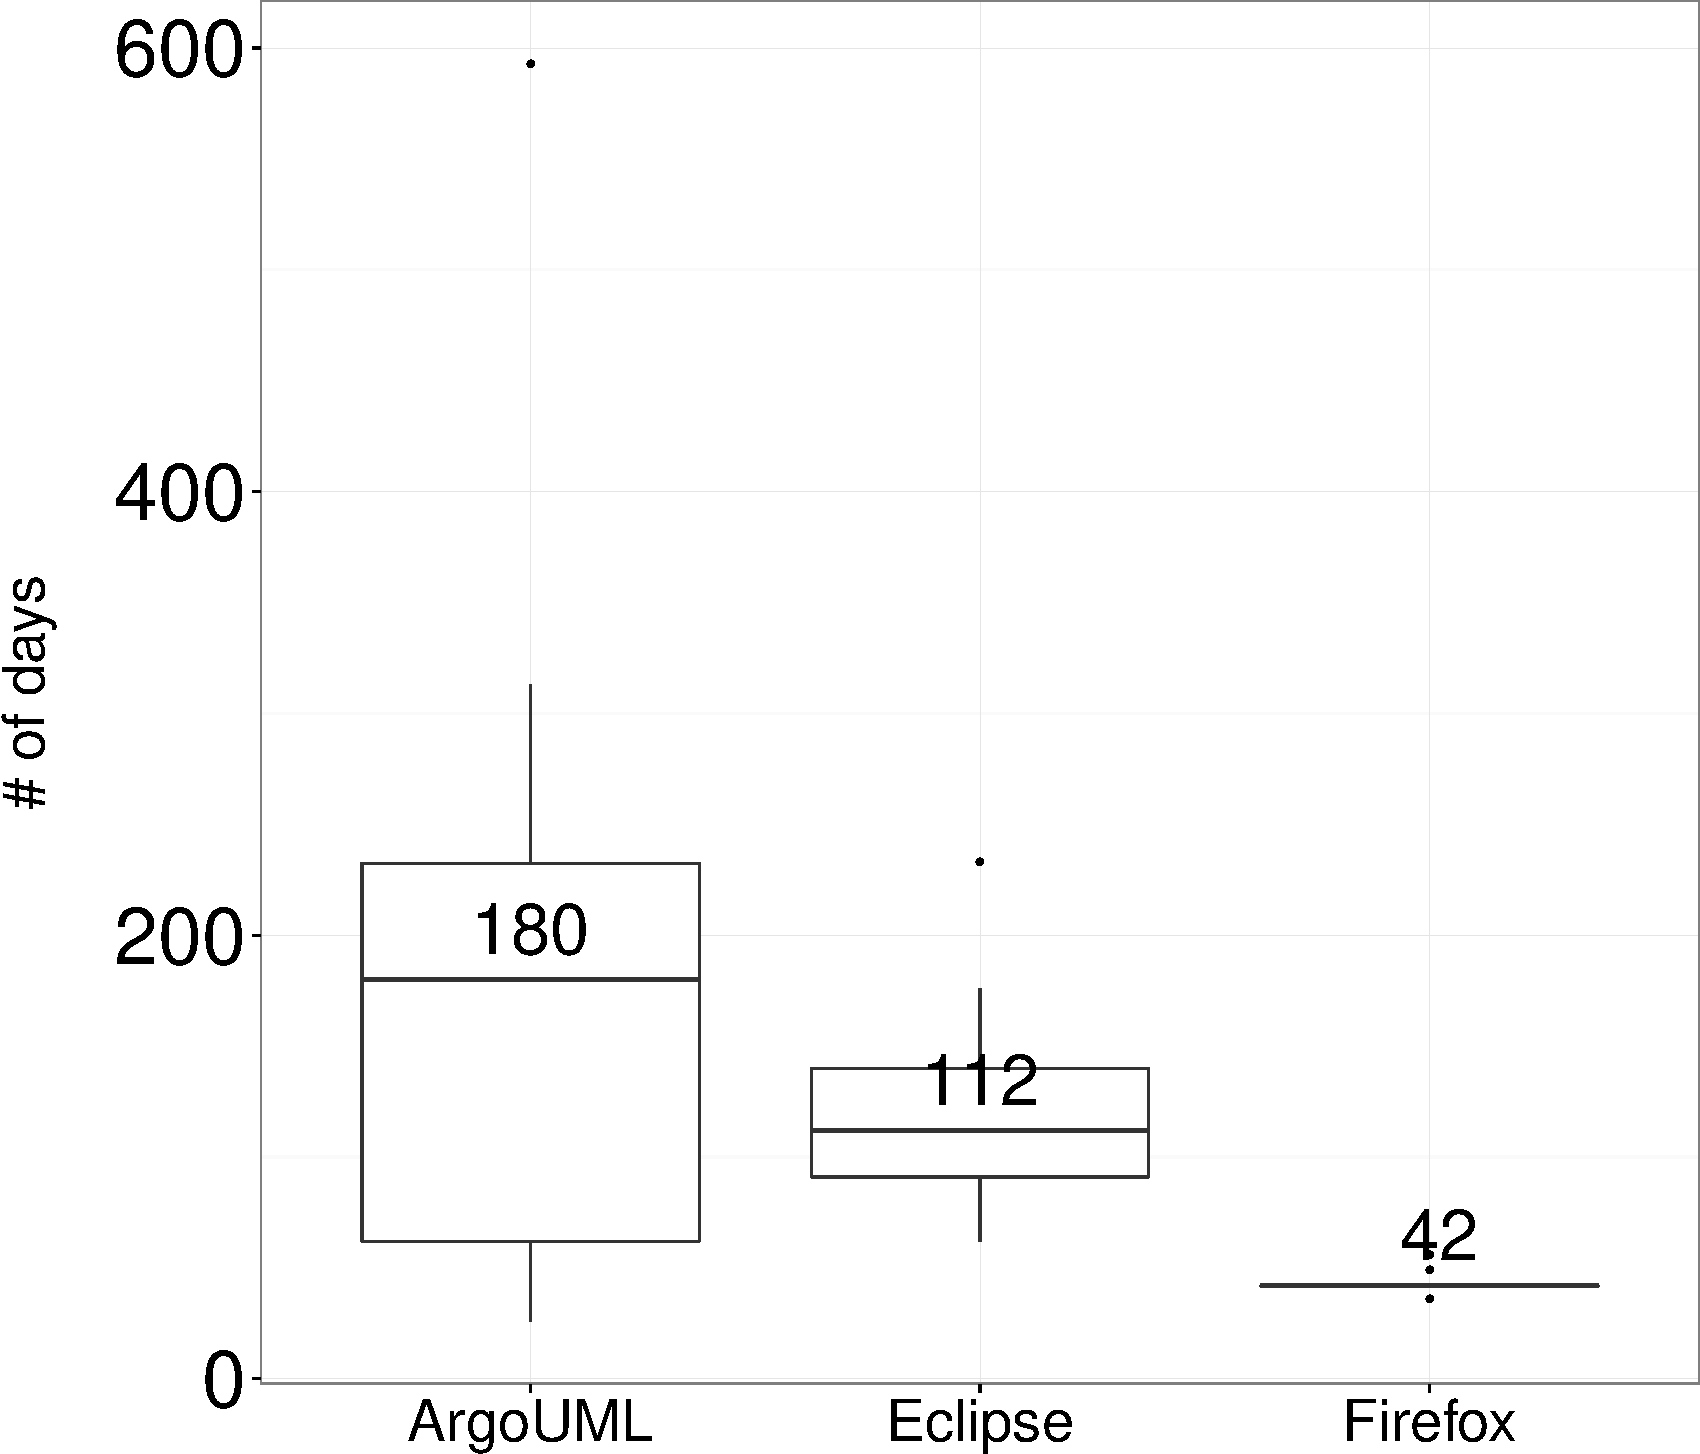
\includegraphics[width=0.7\textwidth]
	{chapters/chapter4/figures/RQ1_time_between_releases.pdf}
	\caption{\textbf{Number of days between the studied releases of the
	ArgoUML, Eclipse, and Firefox projects.} The number shown over each
boxplot is the median interval.}  
	\label{ch4:fig:releaseIntervals}
\end{figure}

\noindent\textit{\textbf{Addressed issues usually
miss the next release in the Firefox project.}}
\hyperref[ch4:fig:releaseIntervals]{Figure}~\ref{ch4:fig:releaseIntervals} shows the
difference between the studied projects in terms of the time interval between
their releases. The median time in days for the Firefox project (42 days) is
approximately $\frac{1}{4}$ that of the ArgoUML project (180 days), and
$\frac{1}{3}$ that of the Eclipse project (112 days). Unlike the Eclipse and
Firefox projects, the distribution for the ArgoUML project is skewed. In
addition, \hyperref[ch4:fig:fixToIntegration]{Figure}~\ref{ch4:fig:fixToIntegration}
shows that the vast majority of addressed issues for the Firefox project is integrated
\textit{after-2} releases, whereas for the Eclipse and ArgoUML projects, the
majority is integrated in the \textit{next} release. 

The reason for the difference may be due to the release policies that are
followed in each project. For example,
\hyperref[ch4:fig:releaseIntervals]{Figure}~\ref{ch4:fig:releaseIntervals} shows that
the Firefox project releases consistently every 42 days (six weeks), whereas the
time intervals between the releases of the ArgoUML project vary from 50 to 220
days. Indeed, the release guidelines for the ArgoUML project state that the
ArgoUML team should release at least one stable release every 8 months (see
\hyperref[argouml:releng]{Section}~\ref{argouml:releng}). The delivery
consistency of the Firefox releases might lead to addressed issues being prevented
from a greater number of releases, since the Firefox project rigidly adhere to a
six-week release schedule despite accumulating issues that could not be
integrated (see \hyperref[firefox:releng]{Section}~\ref{firefox:releng}). 

Although an addressed issue usually misses the next release in the Firefox
project, issues are usually shipped faster when compared to the other projects.
Indeed, \hyperref[ch4:fig:beanplot_days]{Figure}~\ref{ch4:fig:beanplot_days} shows that
addressed issues in the Firefox project take a median of 107 days to be
released, while it takes 166 and 146 days in the Eclipse and ArgoUML projects,
respectively.\\

\noindent\textit{\textbf{34\% to 60\% of addressed issues had their integration
prevented from at least one release in the traditionally released projects.}}
\hyperref[ch4:fig:fixToIntegration]{Figure}~\ref{ch4:fig:fixToIntegration} shows that
98\% of the addressed issues in the Firefox project are prevented from integration
in at least one release. However, for the projects that adopt a more traditional
release cycle, \ie the ArgoUML and Eclipse projects, 34\% to 60\%  of the addressed
issues are prevented from integration in at least one release. This result
indicates that even though an issue is addressed, integration may be prevented by
one or more releases, which can frustrate end users.\\

\begin{figure}[!t]
	\centering
	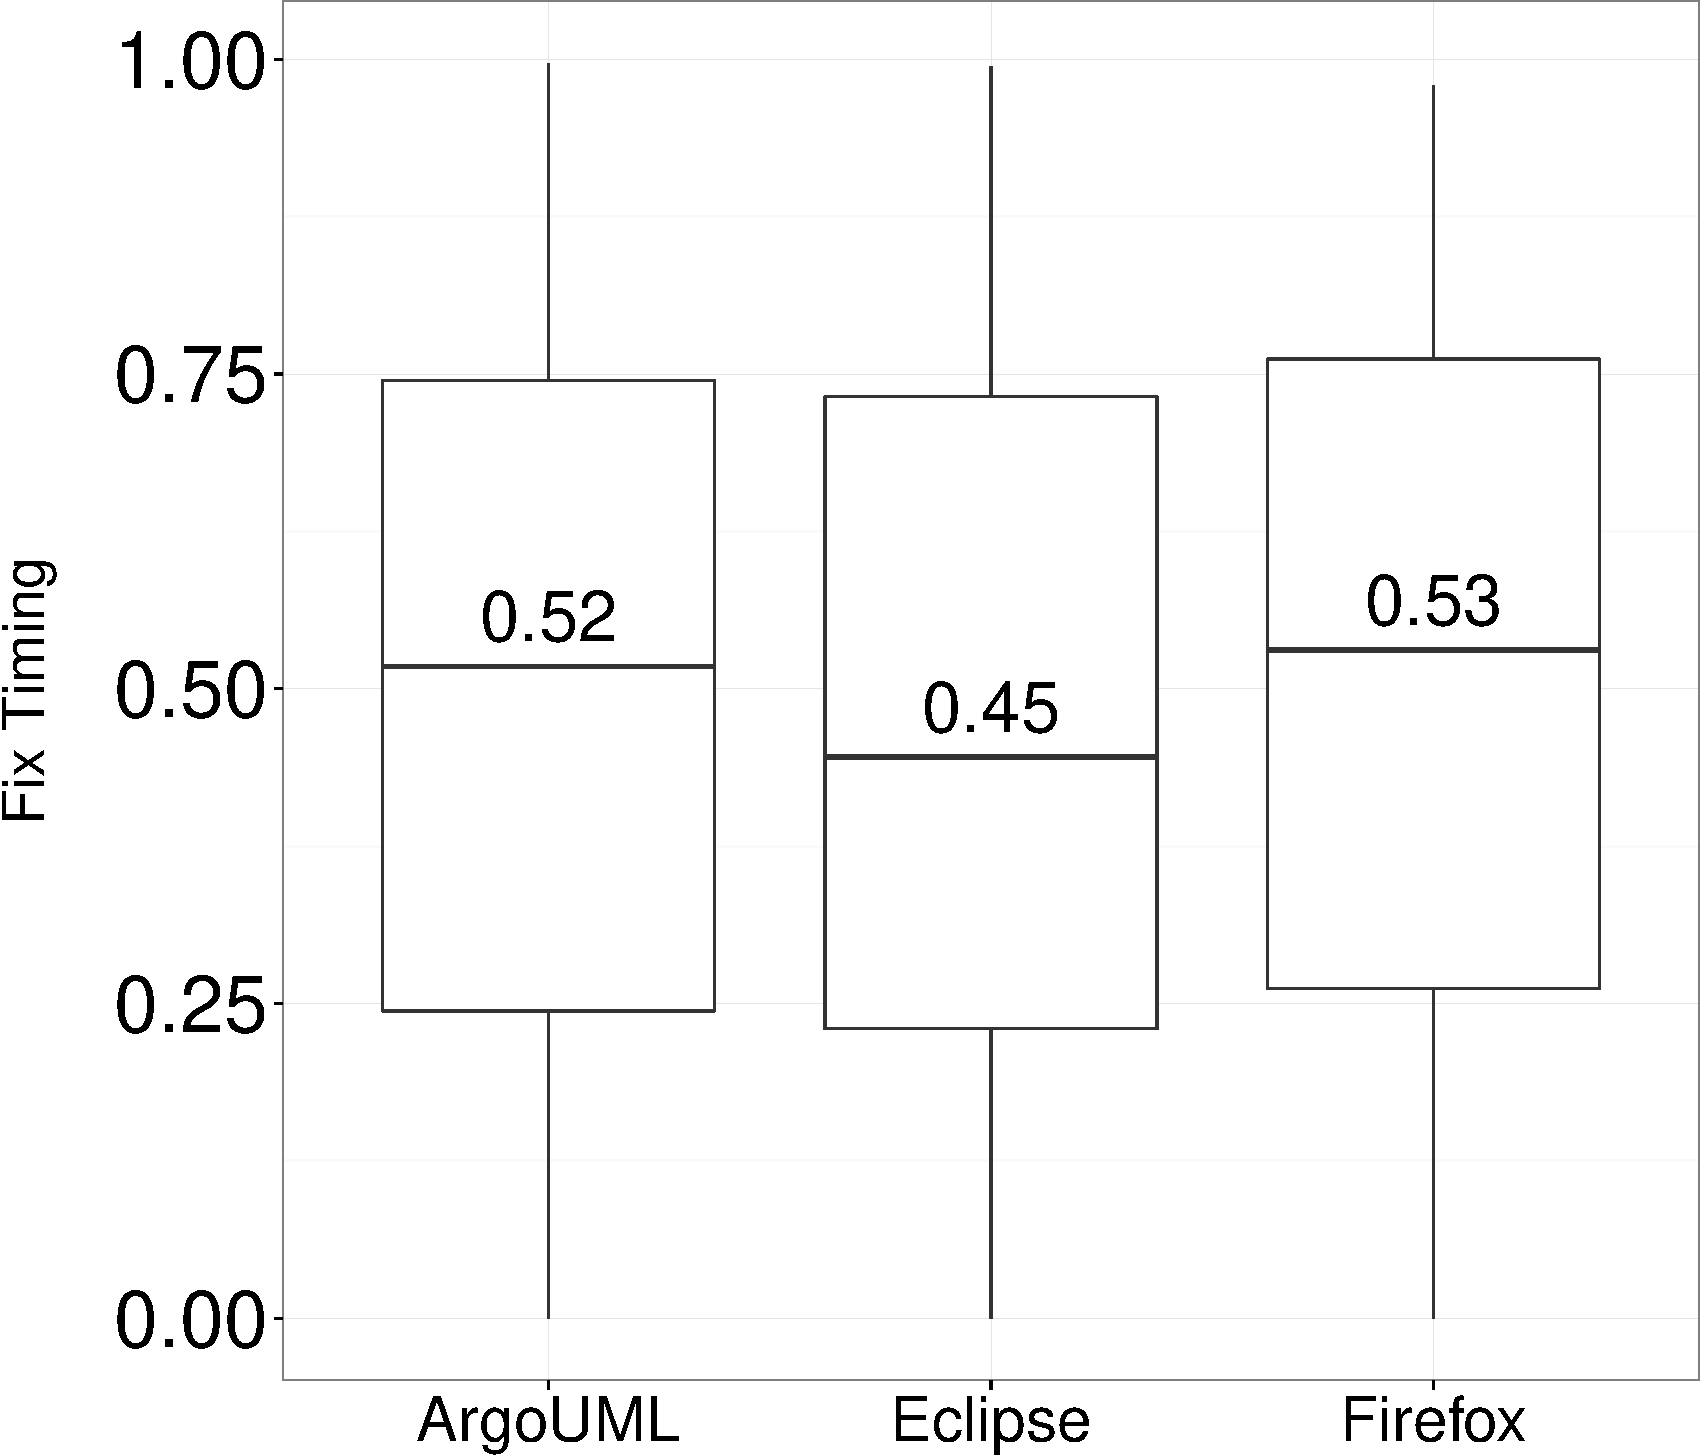
\includegraphics[width=0.7\textwidth]
	{chapters/chapter4/figures/addressing_stage.pdf}
	\caption{\textbf{Fix timing metric.} We present the
		distribution of the \textit{fix timing} metric for addressed
		issues that are prevented from integration in at least one release.}
	\label{ch4:fig:boxplotTimeWindow}
\end{figure}

\noindent\textit{\textbf{Many issues that were prevented from integration are
addressed well before the upcoming release date.}} addressed issues could be prevented
from integration because they were addressed late in the release cycle, \eg one day
or one week before the upcoming release date. To check whether addressed issues are
being prevented from integration mostly because they are being addressed late in the
release cycle, we compute the \textit{fix timing} metric. 

\hyperref[ch4:fig:boxplotTimeWindow]{Figure}~\ref{ch4:fig:boxplotTimeWindow} shows the
distribution of the \textit{fix timing} metric for each project. The smallest
\textit{fix timing} median is observed for the Eclipse project, which is 0.45.
For the ArgoUML and Firefox projects, the median is 0.52 and 0.53, respectively.
The \textit{fix timing} medians are roughly in the middle of the release.
Moreover, the boxes extend to cover between 0.25 and 0.75. The result suggests
that, in the studied projects, issues that are prevented from integration are
usually addressed $\frac{1}{4}$ to $\frac{3}{4}$ of the way through a release.
Hence, it is unlikely that most addressed issues are prevented from integration
solely because they were addressed too close to an upcoming release date.

\conclusionbox{The integration of 34\% to 60\% of the addressed issues in the
	traditionally released projects and 98\% in the rapidly released project
	were prevented from integration in at least one release. Furthermore, we
	find that many issues which integration was prevented, were addressed well
before the releases from which they were omitted.}

